\documentclass[12pt]{article}
\usepackage[all, stdclass]{lix}
\usepackage{graphicx}
\usepackage{svg}
\usepackage{pgfplots}
\svgsetup{
  inkscapepath=assets/,  % Path to the directory containing your SVG files
  svgpath=assets/        % Path to the directory containing your SVG files
}
\usepackage{float}
\usepackage{hyperref}
\usepackage{url}
\usepackage{times}
\usepackage{amsmath}
\usepackage{enumitem}
\usepackage{subcaption}
\usepackage{tikz}
\setlist{topsep=0pt, leftmargin=*}
%----------EDIT COVER INFO HERE -----------------%
\def \LOGOPATH {assets/birzeit-logo.png}
\def \DEPARTEMENT {Department of Electrical \& Computer Engineering}
\def \COURSENUM {ENEE4113}
\def \COURSENAME {Communications Laboratory}
\def \REPORTTITLE {Frequency Modulation}
\def \STUDENTNAME {Mohammad Abu-Shelbaia}
\def \STUDENTID {1200198}
\def \INSTRUCTOR {Dr. Ibrahim Nemer}
\def \ASSISTANT {Eng. Mohammad Al-Battat}
\def \REPORTNUM {4}

\begin{document}
\pagenumbering{Roman}

\begin{titlepage}
    \vfill
    \begin{center}
        \includegraphics[width=0.7\textwidth]{\LOGOPATH} \\
        \hfill \\
        \Large{\DEPARTEMENT} \\
        \Large{\COURSENUM\;-\;\COURSENAME} \\
        \vfill
        \textbf{\LARGE{Experiment \#\REPORTNUM}} \\
        \textbf{\LARGE{\REPORTTITLE}}
    \end{center}
    \vfill
    \begin{flushleft}
        \Large{\textbf{Prepared by:}\\ \STUDENTNAME\quad\STUDENTID} \\

        \Large{\textbf{Instructor:} \INSTRUCTOR} \\
        \Large{\textbf{Assistant:} \ASSISTANT} \\
        \Large{\textbf{Section:} 4}\\
        \LARGE{\textbf{ }}\\
        \LARGE{\textbf{ }}\\
        \LARGE{\textbf{ }}\\
        \Large{\textbf{Date:} \today}\\
    \end{flushleft}
    \vfill
\end{titlepage}


%--------------- TABLES --------------------------------%
\tableofcontents
\clearpage
\setlength{\parskip}{\baselineskip}%
\listoffigures
\clearpage
\listoftables
\clearpage
\pagenumbering{arabic}
%-------------- CONTENT ---------------------%
\h{Theory}
\hh{Modulation Scheme}
Frequency modulation is a part of angle modulation, angle modulation is a technique with constant carrier amplitude and varring phase or time derviative of phase. an FM signal can be expressed as:
\begin{equation}
    s(t) = A_c \cos({\omega}_c t + 2\pi k_f\int_{-\infty}^{t}m(\tau)\,d\tau)
\end{equation}
\begin{itemize}
    \item $A_c$ is the carrier amplitude
    \item ${\omega}_c$ is the carrier frequency
    \item $k_f$ is the modulation sensitivity
    \item $m(t)$ is the message signal
\end{itemize}
\begin{figure}[H]
    \centering
    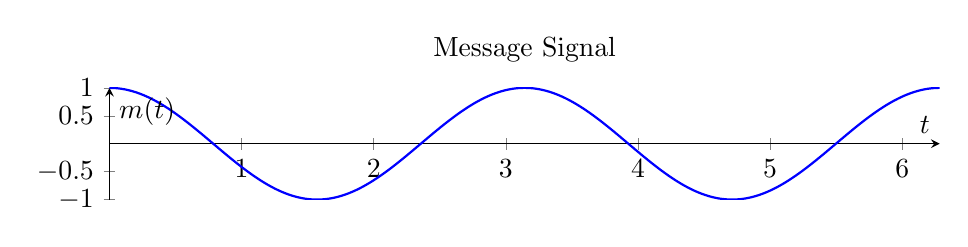
\begin{tikzpicture}
        \begin{axis}[
            width=1\textwidth,
            height=3cm,
            xlabel={$t$},
            ylabel={$m(t)$},
            domain=0:2*pi,
            samples=500,
            axis lines=middle,
            title={Message Signal},
            legend style={at={(0.5,-0.3)},anchor=north},
        ]
        \addplot[blue, thick] {cos(deg(2*x))};
        \end{axis}
    \end{tikzpicture}
    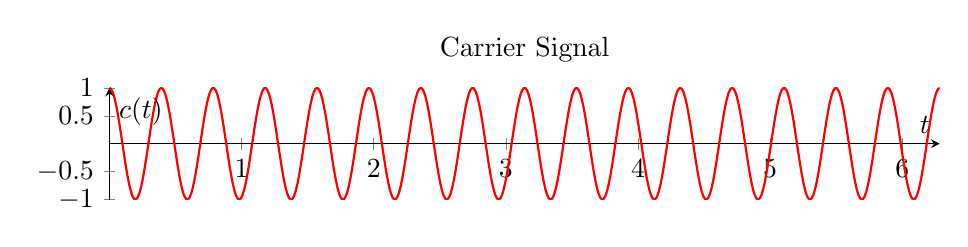
\begin{tikzpicture}
    \begin{axis}[
        width=1\textwidth,
        height=3cm,
        xlabel={$t$},
        ylabel={$c(t)$},
        domain=0:2*pi,
        samples=500,
        axis lines=middle,
        title={Carrier Signal},
        legend style={at={(0.5,-0.3)},anchor=north},
    ]
    \addplot[red, thick] {cos(deg(16*x))};
    \end{axis}
    \end{tikzpicture}
    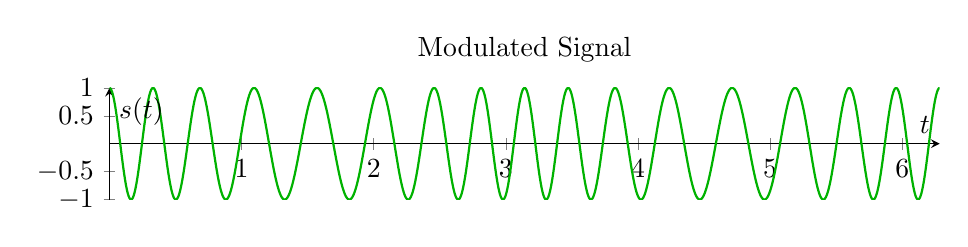
\begin{tikzpicture}
        \begin{axis}[
            width=1\textwidth,
            height=3cm,
            xlabel={$t$},
            ylabel={$s(t)$},
            domain=0:2*pi,
            samples=1000,
            axis lines=middle,
            title={Modulated Signal},
            legend style={at={(0.5,-0.2)},anchor=north},
        ]
        \addplot[green!70!black, thick] {cos(deg(16*x) + 2*pi*15*sin(deg(2*x)))}; % fc = 1, Kf = 64
        \end{axis}
        \end{tikzpicture}
    \caption{Frequency Modulation Scheme}
\end{figure}
\hhh{Modulation}
There is two types of modulation, narrowband and wideband. narrowband modulation is when the modulation index is less than 1, and wideband modulation is when the modulation index is greater than 1. the modulation index is defined as:
\begin{equation}
    \beta = \frac{\Delta f}{f_m} = \frac{k_f A_m}{f_m}
\end{equation}
The simplict way of generating an FM signal is using a voltage controlled oscillator, which is not a stable method. the other method is generating a narrowband FM signal and then using a frequency multiplier to generate a wideband FM signal.

\begin{figure}[H]
    \centering
    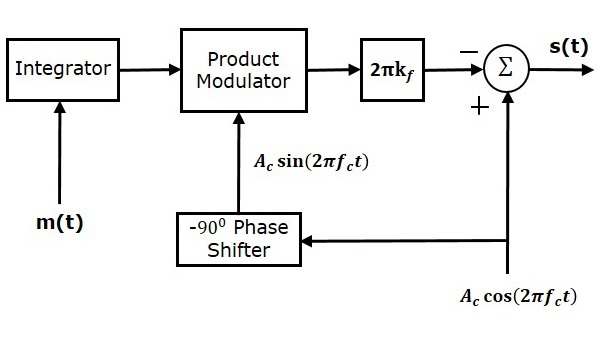
\includegraphics[width=0.5\textwidth]{assets/img/nbfm_modulator.jpg}
    \caption{Narrowband FM Generation}
    \cite{tutorialspoint}
\end{figure}
\begin{figure}[H]
    \centering
    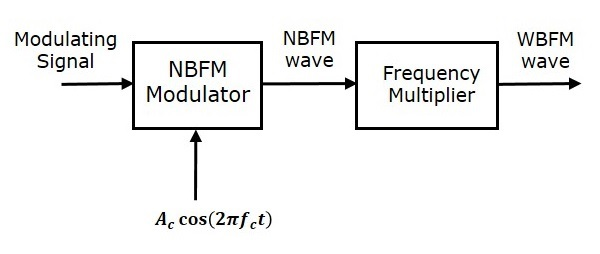
\includegraphics[width=0.5\textwidth]{assets/img/indirect_method.jpg}
    \caption{Wideband FM Generation}
    \cite{tutorialspoint}
\end{figure}
\hhh{Demodulation - Phase Locked Loop}
For demodulation, a common method is the phase locked loop (PLL) a feedback system that synchronizes the phase of the output signal with the phase of the input signal. The phase detector compares the phase of the input signal with the phase of the output signal and generates an error signal that is used to adjust the phase of the output signal. The output of the phase detector is filtered using a low-pass filter to remove high-frequency components, resulting in a demodulated signal.
\begin{figure}[H]
    \centering
    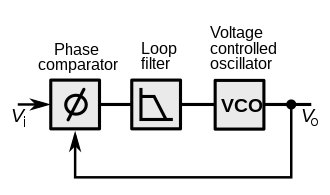
\includegraphics[width=0.5\textwidth]{assets/img/PLL.png}
    \caption{Phase Locked Loop}
\end{figure}
\hhh{Demodulation - Zero Crossing Detector}
A Zero-Crossing FM Detector is a signal demodulation technique that recovers the original information from an FM modulated signal by detecting the points where the signal changes direction. The frequency deviation of the FM signal can be estimated by detecting these zero-crossings, or the points where the signal changes direction, since the frequency of an FM signal is directly proportional to the rate of change of the phase of the signal. This allows for the extraction of the original information.\cite{eecite}
\hh{Carson's Rule}
Carson's rule is a rule of thumb that gives the approximate bandwidth of an FM signal. It states that A 98\% power B.W of an FM signal can be estimated by:
\begin{equation}
    B_T \approx 2(\beta + 1)f_m
\end{equation}
The rule works well when the message signal is continuous. However, it cannot be used when the message contains discontinuities, such as in the case of a square function. \cite{tutorialspoint}
\hh{Besel Functions}
A more accurate expression for the FM signal bandwidth can be obtained using Bessel functions. The FM signal can be expressed as:
\begin{equation}
    s(t) = A_c \cos({\omega}_c t + \beta\sin({\omega}_m t))
\end{equation} 
where $\beta$ is the modulation index, and ${\omega}_m$ is the message signal frequency. In terms of Bessel functions, the FM signal can be expressed as:
\begin{equation}
    s(t) = A_c \sum_{n=-\infty}^{\infty} J_n(\beta) \cos({\omega}_c t + n{\omega}_m t)
\end{equation}
In order to find the bandwidth of the FM signal that achives a certain percentage of the total power, the following equation can be used:
\begin{equation}
    J_0^{2}(\beta) + 2\sum_{n=1}^{m} J_n^{2}(\beta) = p
\end{equation}
where $p$ is the percentage of the total power, and $m$ is the number of bessel functions to be summed, the bandwidth of the FM signal can be calculated using:
\begin{equation}
    B_T = 2*m*f_m
\end{equation}
\clearpage
\h{Procedure}
\h{Data and Calculations}
\h{Conclusion}
\clearpage
\end{document}





